% !TeX root = ../Book2.tex
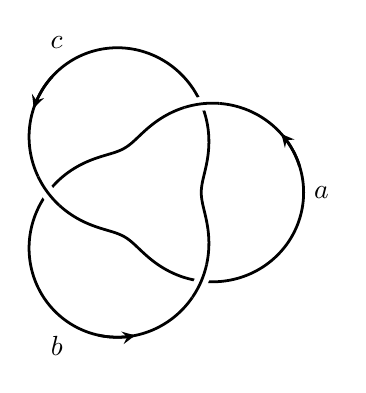
\begin{tikzpicture}[scale=.65,line width=1pt,>=stealth]
	\draw[smooth,samples=361,domain=0:360,variable=\t] plot ({(2+cos(3*\t))*cos(2*\t)},{(2+cos(3*\t))*sin(2*\t)});
	\foreach \tstart/\tend in {26/34,146/154,266/274}{
		\draw[preaction={draw=white,line width=5pt},smooth,samples=15,domain=\tstart:\tend,variable=\t] plot ({(2+cos(3*\t))*cos(2*\t)},{(2+cos(3*\t))*sin(2*\t)});
	}
	\foreach \tstart/\tend in {5/12,125/132,245/252}{
		\draw[->,smooth,samples=12,domain=\tstart:\tend,variable=\t] plot ({(2+cos(3*\t))*cos(2*\t)},{(2+cos(3*\t))*sin(2*\t)});
	}
	\node[right] at (3,0) {\(a\)};
	\node[below left] at (-1.5,-2.6) {\(b\)};
	\node[above left] at (-1.5,2.6) {\(c\)};
\end{tikzpicture}
